\documentclass[a4paper,14pt]{extreport}
\usepackage[left=1.5cm,right=1.5cm,
    top=1.5cm,bottom=2cm,bindingoffset=0cm]{geometry}
\usepackage{scrextend}
\usepackage[T1,T2A]{fontenc}
\usepackage[utf8]{inputenc}
\usepackage[english,russian,ukrainian]{babel}
\usepackage{tabularx}
\usepackage{amssymb}
\usepackage{color}
\usepackage{amsmath}
\usepackage{mathrsfs}
\usepackage{listings}
\usepackage{graphicx}
\graphicspath{ {./images/} }
\usepackage{lipsum}
\usepackage{xcolor}
\usepackage{hyperref}
\usepackage{tcolorbox}
\usepackage{tikz}
\usepackage{ulem}
\usepackage[framemethod=TikZ]{mdframed}
\usepackage{wrapfig,boxedminipage,lipsum}
\mdfdefinestyle{MyFrame}{%
linecolor=blue,outerlinewidth=2pt,roundcorner=20pt,innertopmargin=\baselineskip,innerbottommargin=\baselineskip,innerrightmargin=20pt,innerleftmargin=20pt,backgroundcolor=gray!50!white}
 \usepackage{csvsimple}
 \usepackage{supertabular}
\usepackage{pdflscape}
\usepackage{fancyvrb}
%\usepackage{comment}
\usepackage{array,tabularx}
\usepackage{colortbl}

\usepackage{varwidth}
\tcbuselibrary{skins}
\usepackage{fancybox}
\usepackage{spreadtab}
 % Цвета для гиперссылок
\definecolor{linkcolor}{HTML}{799B03} % цвет ссылок
\definecolor{urlcolor}{HTML}{799B03} % цвет гиперссылок


\usepackage{tikz}
\usepackage[framemethod=TikZ]{mdframed}
\usepackage{xcolor}
\usetikzlibrary{calc}
\makeatletter
\newlength{\mylength}
\xdef\CircleFactor{1.1}
\setlength\mylength{\dimexpr\f@size pt}
\newsavebox{\mybox}
\newcommand*\circled[2][draw=blue]{\savebox\mybox{\vbox{\vphantom{WL1/}#1}}\setlength\mylength{\dimexpr\CircleFactor\dimexpr\ht\mybox+\dp\mybox\relax\relax}\tikzset{mystyle/.style={circle,#1,minimum height={\mylength}}}
\tikz[baseline=(char.base)]
\node[mystyle] (char) {#2};}
\makeatother

\definecolor{ggreen}{rgb}{0.4,1,0}
\definecolor{rred}{rgb}{1,0.1,0.1}
\definecolor{amber}{rgb}{1.0, 0.75, 0.0}
\definecolor{babyblue}{rgb}{0.54, 0.81, 0.94}
\definecolor{amethyst}{rgb}{0.6, 0.4, 0.8}

\usepackage{float}
\usepackage{wrapfig}
\usepackage{framed}
%for nice Code{
\lstdefinestyle{customc}{
  belowcaptionskip=1\baselineskip,
  breaklines=true,
  frame=L,
  xleftmargin=\parindent,
  language=C,
  showstringspaces=false,
  basicstyle=\small\ttfamily,
  keywordstyle=\bfseries\color{green!40!black},
  commentstyle=\itshape\color{purple!40!black},
  identifierstyle=\color{blue},
  stringstyle=\color{orange},
}
\lstset{escapechar=@,style=customc}
%
  % Цвета для гиперссылок
  \definecolor{linkcolor}{rgb}{0, 0.72, 0.92} % цвет ссылок
  \definecolor{urlcolor}{rgb}{0.0, 0.0, 1.0}% цвет гиперссылок
  \hypersetup{pdfstartview=FitH,  linkcolor=linkcolor,urlcolor=urlcolor,citecolor=red, colorlinks=true}



\begin{document}
\pagecolor{white}

%----------------------------------------1
\newtcbox{\xmybox}[1][red]{on line, arc=7pt,colback=#1!10!white,colframe=#1!50!black, before upper={\rule[-3pt]{0pt}{10pt}},boxrule=1pt, boxsep=0pt,left=6pt,right=6pt,top=2pt,bottom=2pt}

\begin{titlepage}
  \begin{center}
    \large
    Національний технічний університет України \\ "Київський політехнічний інститут імені Ігоря Сікорського"


    Факультет Електроніки

    Кафедра мікроелектроніки
    \vfill

    \textsc{ЗВІТ}\\

    {\Large Про виконання лабораторної роботи №1\\
      з дисципліни: «ФУНКЦІОНАЛЬНА ЕЛЕКТРОНІКА»\\[1cm]

        Дослідження динамічних характеристик оптронів


    }
  \bigskip
\end{center}
\vfill

\newlength{\ML}
\settowidth{\ML}{«\underline{\hspace{0.4cm}}» \underline{\hspace{2cm}}}
\hfill
\begin{minipage}{1\textwidth}
Виконавець:\\
Студент 4-го курсу \hspace{4cm} $\underset{\text{(підпис)}}{\underline{\hspace{0.2\textwidth}}}$  \hspace{1cm}А.\,С.~Мнацаканов\\
\vspace{1cm}

Перевірив: \hspace{6.1cm} $\underset{\text{(підпис)}}{\underline{\hspace{0.2\textwidth}}}$  \hspace{1cm}С.\,В.~Малютa\\

\end{minipage}

\vfill

\begin{center}
2021
\end{center}
\end{titlepage}



\newpage
\setcounter{page}{2}



Mета - Дослідження характеристик оптронів та функціональних пристроїв на їх
основі. Дослідження динамічних характеристик оптронів.\


 \begin{figure}[h!]
\center{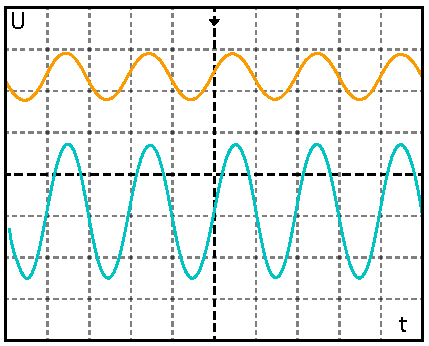
\includegraphics[width=0.7\linewidth]{11.png}}
\caption{Макет для дослідження статичних характеристик оптронів.}
  
\end{figure}


\begin{center}
ПОРЯДОК ВИКОНАННЯ РОБОТИ
\end{center}
\begin{enumerate}
\item Провести вимірювання статичних характеристик оптрона.
\item  Зібрати схему для вимірювання статичних характеристик оптронів
\item  Переключити мультиметр у режим вимірювання опору.
\item  Ввімкнути пару білий світлодіод – фоторезистор та зняти передавальну
характеристику резистивного оптрона при зміні напруги на світлодіоді (діапазон
задається викладачем).
\item  Ввімкнути пару червоний світлодіод – фоторезистор та зняти
передавальну характеристику резистивного оптрона при зміні напруги на
світлодіоді (діапазон задається викладачем).
\item  Ввімкнути пару зелений світлодіод – фоторезистор та зняти
передавальну характеристику резистивного оптрона при зміні напруги на
світлодіоді (діапазон задається викладачем).
\item  Переключити мультиметр в режим вимірювання струму.
\item  Ввімкнути пару білий світлодіод – фотодіод та зняти передавальну
характеристику діодного оптрона при зміні напруги на світлодіоді (діапазон
задається викладачем).
\item  Ввімкнути пару червоний світлодіод – фотодіод та зняти передавальну
характеристику діодного оптрона при зміні напруги на світлодіоді (діапазон
задається викладачем).
\item  Ввімкнути пару зелений світлодіод – фотодіод та зняти передавальну
характеристику діодного оптрона при зміні напруги на світлодіоді (діапазон
задається викладачем).
\item  Вимкнути мультиметр та джерело струму.
\end{enumerate}

\begin{center}
ЕКСПЕРИМЕНТАЛЬНІ РЕЗУЛЬТАТИ
\end{center}
\begin{table}[h!]
\caption{Експериментальні результати ( ФР – фоторезистор, ФД – фотодіод, свд – світлодіод.)}
\begin{tabular}{|ccc|ccc|ccc|}
\hline
\multicolumn{3}{|c|}{ФР – білий СВД}                                & \multicolumn{3}{c|}{ФР – зелений СВД}                             & \multicolumn{3}{c|}{ФР – червоний СВД}                            \\ \hline
\multicolumn{1}{|c|}{Uвх, В} & \multicolumn{1}{c|}{R, кОм} & І, мА  & \multicolumn{1}{c|}{Uвх, В} & \multicolumn{1}{c|}{R, кОм} & І, мА & \multicolumn{1}{c|}{Uвх, В} & \multicolumn{1}{c|}{R, кОм} & І, мА \\ \hline
\multicolumn{1}{|c|}{1.5}    & \multicolumn{1}{c|}{10.44}  & 0.001  & \multicolumn{1}{c|}{1.3}    & \multicolumn{1}{c|}{16.3}   & 0.001 & \multicolumn{1}{c|}{1.1}    & \multicolumn{1}{c|}{500}    & 0.043 \\ \hline
\multicolumn{1}{|c|}{1.6}    & \multicolumn{1}{c|}{9.06}   & 0.0032 & \multicolumn{1}{c|}{1.4}    & \multicolumn{1}{c|}{16.2}   & 0.011 & \multicolumn{1}{c|}{1.2}    & \multicolumn{1}{c|}{400}    & 0.055 \\ \hline
\multicolumn{1}{|c|}{1.7}    & \multicolumn{1}{c|}{8.73}   & 0.0051 & \multicolumn{1}{c|}{1.5}    & \multicolumn{1}{c|}{4.57}   & 0.07  & \multicolumn{1}{c|}{1.3}    & \multicolumn{1}{c|}{12.59}  & 0.075 \\ \hline
\multicolumn{1}{|c|}{1.8}    & \multicolumn{1}{c|}{3.4}    & 0.021  & \multicolumn{1}{c|}{1.6}    & \multicolumn{1}{c|}{2.16}   & 0.26  & \multicolumn{1}{c|}{1.4}    & \multicolumn{1}{c|}{1.2}    & 0.15  \\ \hline
\multicolumn{1}{|c|}{1.9}    & \multicolumn{1}{c|}{1.4}    & 0.078  & \multicolumn{1}{c|}{1.7}    & \multicolumn{1}{c|}{1.06}   & 0.78  & \multicolumn{1}{c|}{1.5}    & \multicolumn{1}{c|}{0.88}   & 1.45  \\ \hline
\multicolumn{1}{|c|}{2}      & \multicolumn{1}{c|}{0.9}    & 0.158  & \multicolumn{1}{c|}{1.8}    & \multicolumn{1}{c|}{0.2}    & 0.79  & \multicolumn{1}{c|}{1.6}    & \multicolumn{1}{c|}{0.5}    & 3.3   \\ \hline
\multicolumn{1}{|c|}{2.1}    & \multicolumn{1}{c|}{0.18}   & 6      & \multicolumn{1}{c|}{1.9}    & \multicolumn{1}{c|}{0.18}   & 1.2   & \multicolumn{1}{c|}{1.7}    & \multicolumn{1}{c|}{0.4}    & 3.8   \\ \hline
\multicolumn{1}{|c|}{2.2}    & \multicolumn{1}{c|}{0,15}   & 10     & \multicolumn{1}{c|}{2}      & \multicolumn{1}{c|}{0.10}   & 4.4   & \multicolumn{1}{c|}{1.8}    & \multicolumn{1}{c|}{0.35}   & 4.7   \\ \hline
\multicolumn{1}{|c|}{}       & \multicolumn{1}{c|}{}       &        & \multicolumn{1}{c|}{2.1}    & \multicolumn{1}{c|}{0.04}   & 6.8   & \multicolumn{1}{c|}{1.9}    & \multicolumn{1}{c|}{0.32}   & 5.5   \\ \hline
\multicolumn{1}{|c|}{}       & \multicolumn{1}{c|}{}       &        & \multicolumn{1}{c|}{2.2}    & \multicolumn{1}{c|}{0.01}   & 9.96  & \multicolumn{1}{c|}{2}      & \multicolumn{1}{c|}{0.32}   & 6     \\ \hline
\multicolumn{1}{|c|}{}       & \multicolumn{1}{c|}{}       &        & \multicolumn{1}{c|}{}       & \multicolumn{1}{c|}{}       &       & \multicolumn{1}{c|}{2.1}    & \multicolumn{1}{c|}{0.28}   & 7.2   \\ \hline
\multicolumn{1}{|c|}{}       & \multicolumn{1}{c|}{}       &        & \multicolumn{1}{c|}{}       & \multicolumn{1}{c|}{}       &       & \multicolumn{1}{c|}{2.2}    & \multicolumn{1}{c|}{0.27}   & 8.1   \\ \hline
\end{tabular}
\end{table}

\begin{landscape}
\begin{table}[]
\begin{tabular}{|ccc|ccc|ccc|}
\hline
\multicolumn{3}{|c|}{ФД – білий СВД}                                     & \multicolumn{3}{c|}{ФД – зелений СВД}                                  & \multicolumn{3}{c|}{ФД – червоний СВД}                                 \\ \hline
\multicolumn{1}{|c|}{Uвх, В} & \multicolumn{1}{c|}{Іфд, мкА} & Ісвд , мА & \multicolumn{1}{c|}{Uвх, В} & \multicolumn{1}{c|}{Іф, мкА} & Ісвд , мА & \multicolumn{1}{c|}{Uвх, В} & \multicolumn{1}{c|}{Іф, мкА} & Ісвд , мА \\ \hline
\multicolumn{1}{|c|}{1.3}    & \multicolumn{1}{c|}{0.2}      & 0.001     & \multicolumn{1}{c|}{1.5}    & \multicolumn{1}{c|}{0.3}     & 0.27      & \multicolumn{1}{c|}{1.1}    & \multicolumn{1}{c|}{0.3}     & 0.3       \\ \hline
\multicolumn{1}{|c|}{1.4}    & \multicolumn{1}{c|}{0.3}      & 0.002     & \multicolumn{1}{c|}{1.6}    & \multicolumn{1}{c|}{0.3}     & 0.3       & \multicolumn{1}{c|}{1.2}    & \multicolumn{1}{c|}{0.5}     & 0.49      \\ \hline
\multicolumn{1}{|c|}{1.5}    & \multicolumn{1}{c|}{0.3}      & 0.004     & \multicolumn{1}{c|}{1.7}    & \multicolumn{1}{c|}{1.4}     & 0.38      & \multicolumn{1}{c|}{1.3}    & \multicolumn{1}{c|}{1.8}     & 0.49      \\ \hline
\multicolumn{1}{|c|}{1.6}    & \multicolumn{1}{c|}{0.3}      & 0.004     & \multicolumn{1}{c|}{1.8}    & \multicolumn{1}{c|}{7.2}     & 0.6       & \multicolumn{1}{c|}{1.4}    & \multicolumn{1}{c|}{5.6}     & 1.38      \\ \hline
\multicolumn{1}{|c|}{1.7}    & \multicolumn{1}{c|}{0.3}      & 0.05      & \multicolumn{1}{c|}{1.9}    & \multicolumn{1}{c|}{15}      & 1         & \multicolumn{1}{c|}{1.5}    & \multicolumn{1}{c|}{10.5}    & 2.9       \\ \hline
\multicolumn{1}{|c|}{1.8}    & \multicolumn{1}{c|}{0.5}      & 0.17      & \multicolumn{1}{c|}{2}      & \multicolumn{1}{c|}{44}      & 2.6       & \multicolumn{1}{c|}{1.6}    & \multicolumn{1}{c|}{29}      & 3.7       \\ \hline
\multicolumn{1}{|c|}{1.9}    & \multicolumn{1}{c|}{1}        & 0.43      & \multicolumn{1}{c|}{2.1}    & \multicolumn{1}{c|}{65}      & 4.1       & \multicolumn{1}{c|}{1.7}    & \multicolumn{1}{c|}{40}      & 4.57      \\ \hline
\multicolumn{1}{|c|}{2}      & \multicolumn{1}{c|}{0.9}      & 0.58      & \multicolumn{1}{c|}{2.2}    & \multicolumn{1}{c|}{89}      & 6         & \multicolumn{1}{c|}{1.8}    & \multicolumn{1}{c|}{51}      & 4.57      \\ \hline
\multicolumn{1}{|c|}{2.1}    & \multicolumn{1}{c|}{21}       & 1.25      & \multicolumn{1}{c|}{2.3}    & \multicolumn{1}{c|}{115}     & 8.4       & \multicolumn{1}{c|}{1.9}    & \multicolumn{1}{c|}{63}      & 5.4       \\ \hline
\multicolumn{1}{|c|}{2.2}    & \multicolumn{1}{c|}{87}       & 5.67      & \multicolumn{1}{c|}{}       & \multicolumn{1}{c|}{}        &           & \multicolumn{1}{c|}{2}      & \multicolumn{1}{c|}{74}      & 6.2       \\ \hline
\multicolumn{1}{|c|}{2.3}    & \multicolumn{1}{c|}{133}      & 9.2       & \multicolumn{1}{c|}{}       & \multicolumn{1}{c|}{}        &           & \multicolumn{1}{c|}{2.1}    & \multicolumn{1}{c|}{99}      & 7.9       \\ \hline
\multicolumn{1}{|c|}{}       & \multicolumn{1}{c|}{}         &           & \multicolumn{1}{c|}{}       & \multicolumn{1}{c|}{}        &           & \multicolumn{1}{c|}{2.2}    & \multicolumn{1}{c|}{111}     & 8         \\ \hline
\multicolumn{1}{|c|}{}       & \multicolumn{1}{c|}{}         &           & \multicolumn{1}{c|}{}       & \multicolumn{1}{c|}{}        &           & \multicolumn{1}{c|}{2.3}    & \multicolumn{1}{c|}{124}     & 9.6       \\ \hline
\end{tabular}
\end{table}

  
\end{landscape}

\begin{center}
ОБРОБКА РЕЗУЛЬТАТІВ
\end{center}
Побудовані
 передавальні
характеристики – залежності фотоопору та фотоструму від струму через
світлодіод:
\begin{figure}[h!]
\center{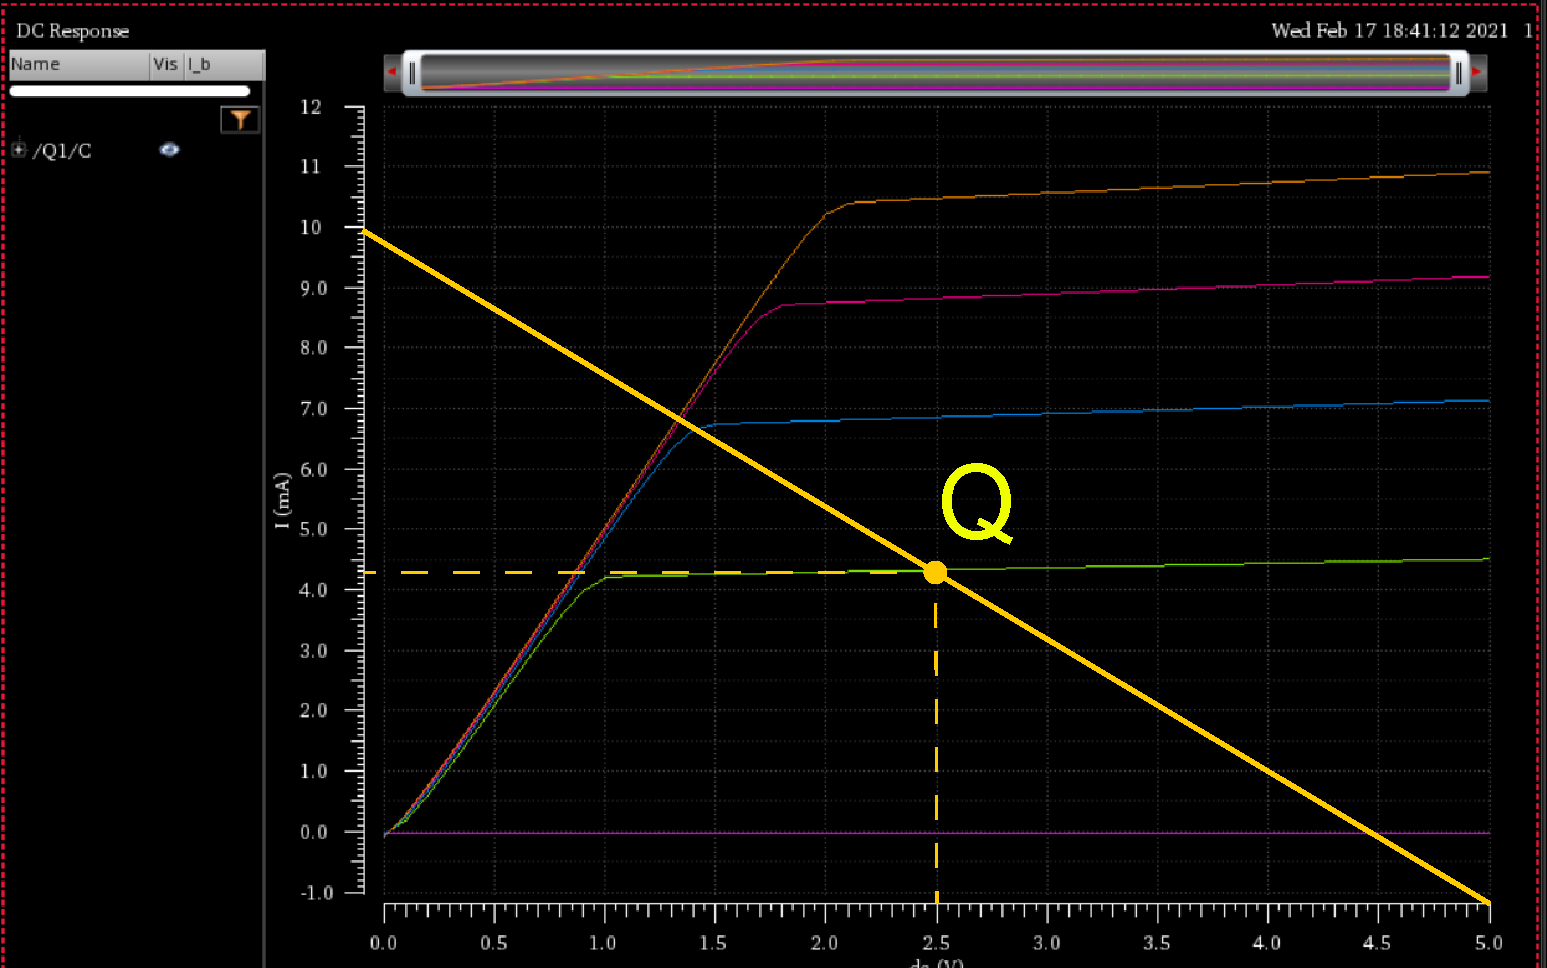
\includegraphics[width=0.7\linewidth]{1.png}}
\caption{Залежність фотоопору від струму через світлодіод для
білого та зеленого світлодіоду}
\end{figure}

 
\begin{figure}[h!]
\center{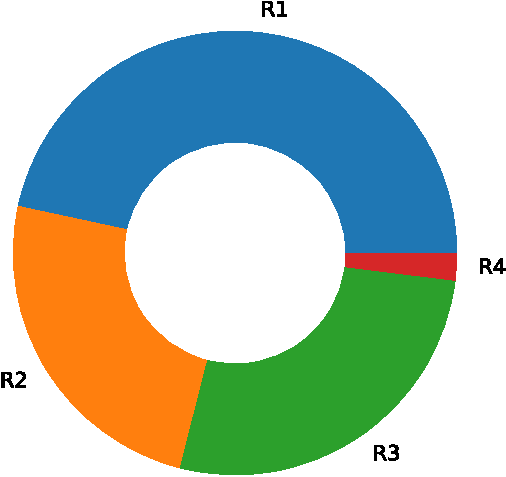
\includegraphics[width=0.7\linewidth]{2.png}}
\caption{Залежність фотоопору від струму через світлодіод для
червоного світлодіоду}
\end{figure}


\begin{figure}[h!]
\center{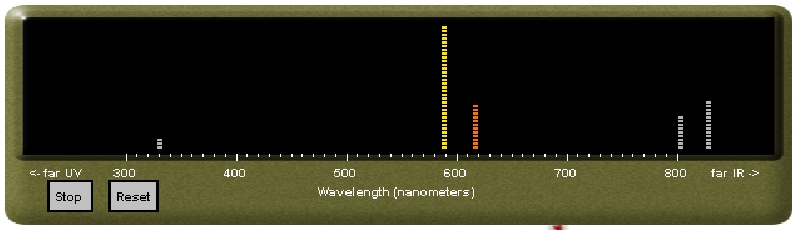
\includegraphics[width=0.7\linewidth]{3.png}}
\caption{Залежність фотоструму від струму через світлодіод для
трьох випадків}
\end{figure}

Коефіцієнт передачі К розрахуємо з формули:\\ 

\begin{equation}
\begin{array}{r}
K=\dfrac{I_{\text{ФД}_{2}}-I_{\text{ФД}_{1}}}{I_{\text{СД}_{2}}-I_{\text{СД}_{1}}} \\
K=\dfrac{I_{\text{ФР}_{2}}-I_{\text{ФР}_{1}}}{I_{\text{СД}_{1}}-I_{\text{СД}_{2}}}
\end{array}
\end{equation}

де ІФД1-2, ІФР1-2 – значення струму, що протікає через світлодіод, обране в лінійній
ділянці передавальної характеристики; ІСД1, ІСД2 – відповідне до обраного
значення струму світлодіоду значення вхідного струму.\\[2cm]



Розрахуємо К для випадку ФД – білий СВД, дані, необхідні для
розрахунку, обираємо із таблиці\\ 
\begin{equation}
K=\dfrac{ 133 - 87}{9,2-5,6  } = 0,0127
\end{equation}

Аналогічно для інших\\ 
Для  ФД – зелений св-да: К = 0,006\\ 
Для  ФД – червоний св-да: К = 0,017\\
Для  ФР – білий св-да:  К = -3688,42 Ом/А.\\
Для  ФР – зелений св-да: K= -9876,74 Ом/А.\\
Для  ФР – червоний св-да: K = -15673,5 Ом/А.\\ 


\begin{center}
ВИСНОВКИ
\end{center}

Оптрон має прямий оптичний зв’язок, для такого типу зв’язку характерно:
1) висока шумозахищеність, оскільки відсутній гальванічний зв'язок між
входом і виходом;
2) можливість керування по кожному з трьох незалежних входів;
3)
 велика
 гнучкість
 та
 можливість
 принципу
 фотоелектронного
перетворення, що створює умови для одержання оптоелектронних схем різного
призначення.
Найбільший коефіцієнт передачі К для пари ФД – червоний світлодіод,
найменший для пари ФД – зелений світлодіод.




\end{document}